% !TEX program = pdflatex
% !TEX encoding = UTF-8 Unicode


\documentclass[linenumbers]{agujournal2019}

\graphicspath{ {figures/} }
%\usepackage{lineno,layouts,microtype}

\usepackage{natbib}

%\linenumbers

\newcommand{\navidcomment}[1]{{\color{red} [#1]}}
\newcommand{\andycomment}[1]{{\color{blue} [#1]}}

%\usepackage[T1]{fontenc}
%\renewcommand*\familydefault{\sfdefault} 
%\usepackage{sansmath} 
%\sansmath

\newcommand{\mathbfit}[1]{\textbf{\textit{\textsf{#1}}}}
\usepackage{amsfonts, amssymb, amsmath}
%\usepackage[labelfont=bf]{caption}

\hypersetup{
	breaklinks,
	colorlinks=true,
	linkcolor=Blue,
  urlcolor=Purple,
	citecolor=Purple,
%	allcolors=black,
 }

 \usepackage{doi}

\usepackage{comment}

\journalname{JGR: Oceans}




\begin{document}
\justify
\title{Circumpolar variations in the chaotic nature of Southern Ocean eddy dynamics}

\authors{
Andrew McC. Hogg\affil{1}, Thierry Penduff\affil{2}, Sally E. Close\affil{2}, William K. Dewar\affil{3},\\Navid C. Constantinou\affil{1}, \quad and\quad Josu{\'e} Mart{\'i}nez Moreno\affil{1}
}

\affiliation{1}{Research School of Earth Sciences and ARC Centre of Excellence for Climate Extremes,\\ Australian National University, Canberra, Australia}
\affiliation{2}{Universit{\'e} Grenoble Alpes, CNRS, IRD, Grenoble-INP, Institut des G{\'e}osciences de l'Environnement (IGE), Grenoble, France}
\affiliation{3}{Florida State University, Tallahassee, FL, USA}

\correspondingauthor{Andrew McC. Hogg}{Andy.Hogg@anu.edu.au}

\begin{keypoints}
\item Variability in the Southern Ocean eddy field is dominated by chaotic, rather than forced, processes.
\item The forced component of the eddy kinetic energy variance is significantly correlated with the local wind stress input.
\item The eddy field lags the wind stress, with two clear timescales emerging: one at $\sim$6 months, which we attribute to baroclinic instability, and one at 2-3 years, which we attribute to the delayed effect of topographic steering.
\end{keypoints}

\begin{abstract}
Circulation in the Southern Ocean is unique.
The strong wind stress forcing and buoyancy fluxes, in concert with the lack of continental boundaries, conspire to drive the Antarctic Circumpolar Current replete with an intense eddy field.
The effect of Southern Ocean eddies on the ocean circulation is significant -- they modulate the momentum balance of the zonal flow, and the meridional transport of tracers and mass.
The strength of the eddy field is controlled by a combination of forcing (primarily thought to be wind stress) and intrinsic, or chaotic, variability associated with the turbulent flow field itself.
Here, we present results from an eddy-permitting ensemble of ocean model simulations to investigate the relative contribution of forcing and intrinsic processes in governing the variability of Southern Ocean eddy kinetic energy.
We find that chaotic processes dominate the eddy field, even on longer timescales.
Where correlations between the forcing and the eddy field exist, these interactions are dominated by two distinct timescales -- a fast baroclinic instability response; and a multi-year process owing to feedback between bathymetry and the mean flow.
These results suggest that understanding Southern Ocean eddy dynamics and its larger-scale impacts requires an ensemble approach to eliminate intrinsic variability, and therefore may not yield robust conclusions from observations alone.

\noindent \textbf{Plain language summary} \\
\noindent The Southern Ocean is the most turbulent part of the world's oceans.
The variations in this turbulence, which is often referred to as \emph{eddies}, is critical to understanding the evolution of the Southern Ocean under climate change.
But it's hard to get information about these eddies, because they occur on small scales in a large ocean basin that is poorly observed.
In addition, the observational record is quite short, which makes it more difficult to use these observations to study what controls variation in the eddy field.
For this reason, we take an eddy-permitting ocean model, and run it 50 times with the same forcing (but a slightly different initial state).
The chaotic nature of the turbulent ocean means that these model runs exhibit different evolutions.
We thus use these simulations to study which eddy processes are intrinsic (that is, a consequence of the chaotic nature of turbulence) and which are forced by the external forcing that is common to all experiments (such as wind forcing).
We conclude that the Southern Ocean eddy field is dominated by intrinsic chaotic processes; but that the forced variability responds to wind on particular timescales that are controlled by the mechanisms that generate ocean turbulence. 
\end{abstract}



%% ------------------------------------------------------------------------ %%
%
%  TEXT
%
%% ------------------------------------------------------------------------ %%

\section{Introduction}

The Southern Ocean is unique in the global ocean; it is the one region without continents on its zonal boundaries, giving rise to the Antarctic Circumpolar Current (ACC) which flows eastward around the globe.
The ACC acts to connect the other major basins and thereby regulates climate and nutrients.
The Southern Ocean region is also a place where mid- and high-latitude ventilation of the oceans occurs, leading to carbon and heat uptake and controlling deep ocean stratification \citep{Rousselet2021, Morrison2022}.
However, the Southern Ocean is also poorly observed (compared with other ocean basins) and its unique properties mean that understanding the dynamics (with the aim of predicting future responses to climate change) need to be urgently constrained.

Another unique feature of the Southern Ocean is that it has a strong eddy field \citep{Fu2010}.
This strong eddy field has been suggested to be important in the Southern Ocean's response to change.
For example, the eddy saturation hypothesis \citep{Hallberg2006, Meredith-Hogg-2006, Munday2013, Constantinou2019} suggests that the role of eddies in facilitating vertical momentum transport acts to limit the response of ACC transport to changing winds.
A similar dynamics, known as eddy compensation, describes the role of eddies in moderating the effect of wind-driven change on the Southern Ocean overturning circulation \citep{Morrison2013a}.
Therefore, the response of fine scale transient motion in the Southern Ocean is likely important to characterising the dynamics of this region.

The strength of the Southern Ocean eddy field is usually characterised by extracting the kinetic energy of transient motions; referred to by oceanographers as eddy kinetic energy (EKE). 
It is important to highlight that EKE includes all transient motion, not just coherent vortices \citep{Martinez-Moreno2019}, and thus care needs to be taken in interpreting this metric.
Eddy kinetic energy has a complex relationship with the forces that drive the ocean circulation.
\citet{Meredith-Hogg-2006} found significant variations in the area-averaged eddy field in some regions, and argued for a 2-3 year lag between events in wind stress forcing and EKE anomalies.
\citet{Patara2016}, using a realistic high-resolution ocean model found that EKE does have a lagged response to wind stress anomalies, but that this relationship is variable around the Southern Ocean.
Idealised models over a wide range of parameter space \citep{Sinha2016} have highlighted that the timescale of the perturbation is critical in determining the EKE response, with shorter perturbations having a faster, Ekman-related response.
Thus, current knowledge suggests that there is a relationship between wind forcing and the Southern Ocean, but that the nature of this relationship needs to be clarified.

On longer timescales it has also been proposed that EKE has increased over recent decades \citep{Hogg2015, Martinez-Moreno2019, Martinez-Moreno2021-ncc}.
The robustness of this wind-EKE relationship in the Southern Ocean was recently investigated by \citet{Zhang2021}, who used crossover data from satellite observations \citep[as in][]{Hogg2015} to better estimate the EKE on regional scales.
When fine graining these calculations it was found that only a single region (30$^\circ$ in longitude) expressed a significant long-term trend in EKE.
This finding  suggests that previous characterisations of the response may have been dominated by a small number of regional events, calling into question the robustness of previous studies.

The dynamical importance of the Southern Ocean eddy field, and uncertainty over the robustness of its variability and trends, motivate a deeper investigation into the processes that control Southern Ocean eddies.
A key issue here is the extent to which the eddy field purely responds to external (atmospheric) forcing, versus the role of chaotic and intrinsic variability in determining eddy energy.
The fact that high-frequency eddy variability is random and chaotic is well-known, and even non-eddying ocean models can also produce (a small amount of) intrinsic variability via large-scale baroclinic instability \citep[e.g.][]{DeVerdiere1999}.
At longer timescales intrinsic variability can emerge from oceanic non-linearities under constant or seasonal forcing and persists under variable forcing \citep{Leroux2018}.
Such intrinsic variabilty has a random phase (that is, it is chaotic in character); it mostly emerges at mesoscale and can cascade toward interannual time scales and O(1000$\,$km) space scales \citep{Serazin-etal-2018}.
One of the goals of this work is characterise the spatiotemporal extent of chaotic, intrinsic, variability in determining  Southern Ocean EKE.

A primary complication in understanding Southern Ocean EKE is the limitation of inference from an admittedly short satellite record; in particular, whether individual events can be attributed to forcing changes, or to intrinsic variability, or a combination of the two.
In this paper, we address this question by examining the intrinsic variability of the Southern Ocean eddy field in an ensemble of eddy-permitting ocean simulations.
We use the OceaniC Chaos – ImPacts, strUcture, predicTability (OCCIPUT) ensemble of global ocean/sea-ice hindcast simulations \citep{Penduff-etal-2014, Leroux2018}, a 50-member ensemble of hindcast simulations.
We examine both the intrinsic variance of the eddy field, and extract the ``forced'' (ensemble mean) component of the variability.
This variability is examined on a circumpolar and regional basis, to better understand the regional differences and processes which contribute to the eddy field.



\section{Methods}

\subsection{The OCCIPUT ensemble}

The methodology employed in this study is derived from the probabilistic approach to ocean modelling outlined by \citet{Bessieres2017}.
We use output from the OCCIPUTensemble of 50 eddy-permitting global ocean--sea ice simulations, based on the ORCA025 implementation \citep[e.g.][]{Barnier2006} of the NEMO modelling system \citep{Madec2012}. 
The model grid has a 1/4$^\circ$ horizontal resolution and 75 geopotential levels. We employ the probabilistic ocean modelling approach outlined by \citet{Bessieres2017}: 
\begin{enumerate}
\item The 50 ensemble members are initialized in 1960 from a single-member 21-year spinup;
\item The ensemble spread is seeded by activating a stochastic perturbation \citep{Brankart-etal-2015} over one year (1960), after which the perturbation is terminated;
\item The 50 ensemble members are driven between 1960 and 2015 by the same realistic atmospheric forcing function based on the ERA-40 and ERA-Interim reanalyses (Drakkar Forcing Set DFS5.2; \citet{Dussin-etal-2016}).
\end{enumerate}
In these simulations the wind stress is computed without ocean current feedbacks, hence ensuring that the same momentum fluxes are applied to all members. 
We focus our analyses on the period 1980-2015, thus yielding an effective spinup duration of 41 years in each member. 


\subsection{Estimating geostrophic eddy velocity}
For each ensemble member, the sea surface height, $\eta_i$, is saved as a 5-daily average (where $i$ represents the ensemble member). 
For each ensemble member, the member's global mean sea level anomaly is subtracted from all grid points at every time step to correct for spurious terms introduced by the use of the Boussinesq approximation \citep{Greatbatch1994}. 
The model drift, which is potentially nonlinear, is then corrected for by detrending using a LOWESS filter \citep{Cleveland1979} in combination with a 5th-order spline; full details of this preprocessing may be found in \cite{Close2020}.

The sea level anomaly, $\eta_i'$, is calculated as the transient component of sea level, given by 
\begin{linenomath*}
\begin{equation}
\eta_i' = \eta_i - \overline{\eta_i},
\end{equation}
\end{linenomath*}
where $\overline{\cdot}$ represents the temporally filtered sea level \citep{Close2020}.
The sea level anomaly is detrended, and then used to calculate the eddy velocity field.
Surface eddy velocity in each ensemble member, $\mathbf{u}_i' = (u_i', v_i')$ is estimated from the detrended sea level anomaly via the geostrophic relation,
\begin{linenomath*}
\begin{equation}
u_i' = - \frac{g}{f} \frac{\partial \eta_i'}{\partial y} \quad \text{and} \quad v_i' = \frac{g}{f} \frac{\partial \eta_i'}{\partial x},
\end{equation}
\end{linenomath*}
where $g$ is the acceleration due to gravity and $f$ is the local Coriolis parameter.
Anomalous values of $\mathbf{u}_i'$ close to coastlines are removed.

The surface eddy kinetic energy for each ensemble member is calculated as 
\begin{linenomath*}
\begin{equation}
E_i = \frac{1}{2}(u_i'^2 + v_i'^2),
\end{equation}
\end{linenomath*}
and subsampled at monthly temporal resolution.
It is notable that $E_i$ contains a large component of seasonal variation \citep{Martinez-Moreno2021} which dominates the statistics.
To look at the forced response, we therefore deseasonalise $E_i$, by removing the climatological mean for each month.
We then proceed to compute ensemble statistics from this deseasonalised EKE.

\subsection{Ensemble eddy statistics}

The eddy kinetic energy can be averaged over the $N$ ensemble members to give the ensemble mean EKE, written as
\begin{linenomath*}
\begin{equation}
\langle E_i \rangle = \frac{1}{N} \sum_{i=1}^N E_i.
\end{equation}
\end{linenomath*}
The argument can be made that, since each ensemble member is forced with identical atmospheric conditions, the forced EKE response is encapsulated by this ensemble mean quantity.
On the other hand, the intrinsic variability of EKE in each ensemble member is found by taking the difference from the ensemble mean for each member,
\begin{linenomath*}
\begin{equation}
E_i^* = E_i - \langle E_i \rangle,
\end{equation}
\end{linenomath*}
where $\cdot^*$ is used to indicate departure from the ensemble mean.
With these expressions in hand, we follow \citet{Leroux2018} to define the  time-variance of the ensemble-mean EKE,
\begin{linenomath*}
\begin{equation}
\sigma^2_{\langle E \rangle} = \frac{1}{T} \sum_{t=1}^T \left(\langle E_i \rangle -  \overline{\langle E_i \rangle}\right)^2,
\end{equation}
\end{linenomath*}
which represents the variance of the forced eddy response.
Analogously, the intrinsic variance emerges from the variance,
\begin{linenomath*}
\begin{equation}
\epsilon^2(t) = \frac{1}{N} \sum_{i=1}^N E_i^*(t)^2,
\end{equation}
\end{linenomath*}
indicating the spread of each member from the ensemble mean.
The fraction of intrinsic variance is then computed as the ratio of the intrinsic variance to the total variance,
\begin{linenomath*}
\begin{equation}
R_i =  \frac{\overline{\epsilon^2}}{\overline{\epsilon^2} + \sigma^2_{\langle E \rangle}}.
\end{equation}
\end{linenomath*}
When $R_i$ approaches unity, the system is dominated by intrinsic variability, and at the limit  of $R_i \to 0$ the system is solely responding to forced variability induced by atmospheric forcing.

To examine the relationship between the EKE (of either the ensemble mean, or from individual ensemble members) we are guided by previous work which emphasises the role of wind stress in governing the eddy variability at different timescales \citep[e.g.][]{Hogg2015, Sinha2016}.
Thus, we look at the correlation coefficient, $r$, at a range of lags between the wind stress $\tau$ (which is identical for all ensemble members) and EKE.
For each correlation we evaluate the statistical significance of the correlation \citep[following, e.g.][]{Santer2000}.
We first calculate the effective sample size, $N_e$, where
\begin{linenomath*}
\begin{equation}
N_e \equiv N \frac{1-r_1 r_2}{1+r_1 r_2},
\end{equation}
\end{linenomath*}
where $N$ is the total number of samples (444 months for this timeseries), $r_1$ is the lag-1 autocorrelation for EKE and $r_2$ is the lag-2 autocorrelation for wind stress.
We use the Students t-test to infer statistical significance (at the 95\%-level) based on this effective sample size, when
\begin{linenomath*}
\begin{equation}
T = \frac{r \sqrt{N_e}}{\sqrt{1-r^2}} > 2.
\end{equation}
\end{linenomath*}
Lagged correlation estimates indicate when this significance test is satisfied.

\section{Results}

The intensity of the Southern Ocean eddy field is not uniform.
Snapshots of eddy kinetic energy (Fig.~\ref{Fig:1}a) show the occurrence of strong eddies which occur in the lee of subsurface topography and at the outlet from western boundary currents such as the Agulhas retroflection and Malvinas current.
The same patterns are evident in the ensemble and temporal mean of the eddy energy ($\langle\textrm{EKE}\rangle$; Fig.~\ref{Fig:1}b), although the signal of individual eddies is no longer apparent.
The strongest band of $\langle\textrm{EKE}\rangle$ approximately follows the path of the Antarctic Circumpolar Current, and $\langle\textrm{EKE}\rangle$  is weak south of 60$^\circ$S.
The patterns of $\langle\textrm{EKE}\rangle$  in this model broadly match the regional variations of $\langle\textrm{EKE}\rangle$  observed from satellite altimetry, albeit at slightly lower intensity, as expected in an eddy-permitting model \citep[e.g.][]{Kiss2020}.

\begin{figure}[ht]
\begin{center}
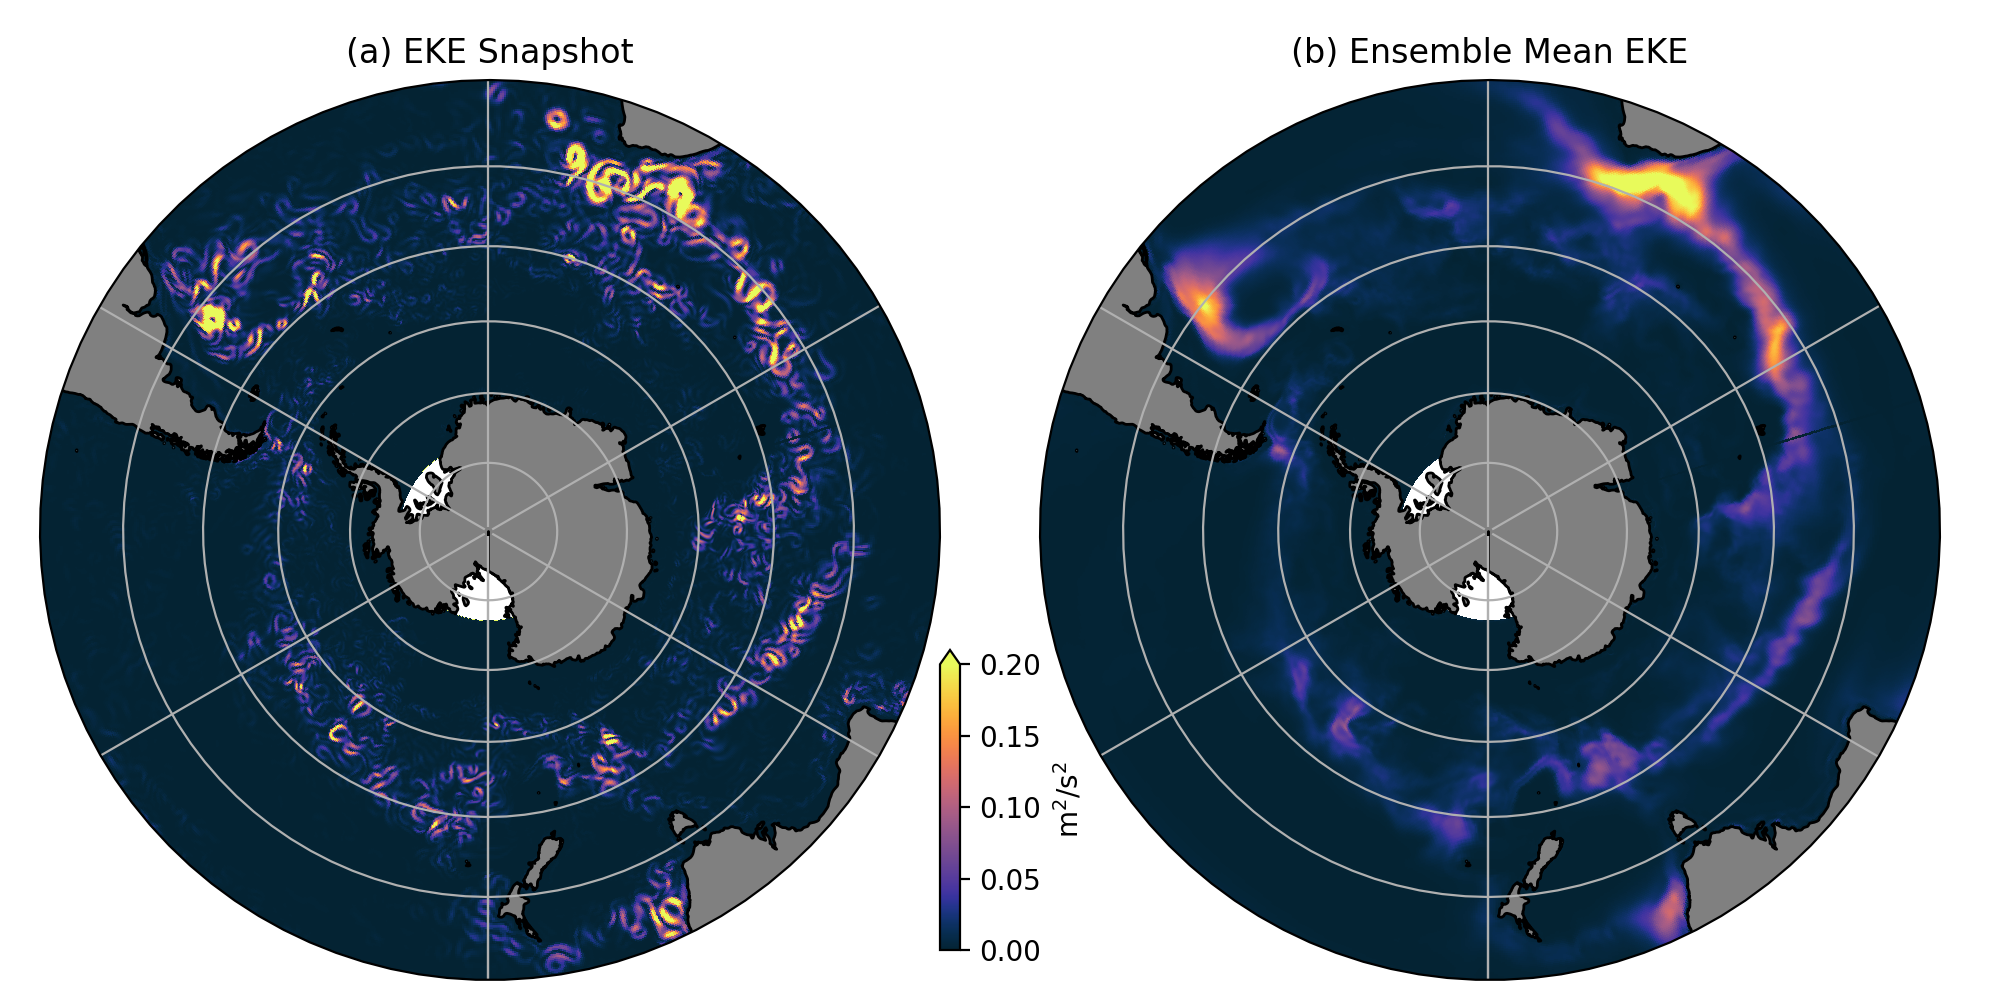
\includegraphics[width=\hsize]{Figure1}
\caption{(a) Snapshot (5-day average) from a single ensemble member showing Southern Ocean EKE, $E_i$, and (b) time-averaged ensemble mean EKE, $\overline{\langle E_i\rangle}$.}
\label{Fig:1}
\end{center}
\end{figure}

For each of the 50 members of the OCCIPUT ensemble we take the EKE averaged over the entire Southern Ocean (40$^\circ$-60$^\circ$S), and plot the deseasonalised EKE anomalies from each ensemble member in thin grey lines in Fig.~\ref{Fig:2}(a). 
This plot highlights the considerable spread in EKE, even when averaged over the full circumpolar belt; in other words, there is a significant component of chaotic (intrinsic) variability in the Southern Ocean eddy field.
Nonetheless, when averaged over all ensemble members (red line in Fig.~\ref{Fig:2}a) the existence of a coherent (forced) component of eddy variability is revealed.
Averaged over this region the fraction, $R_i$, of intrinsic variance is 0.82, confirming the visual impression that intrinsic processes dominate eddy variability in the Southern Ocean eddy field.

\begin{figure}[t]
\begin{center}
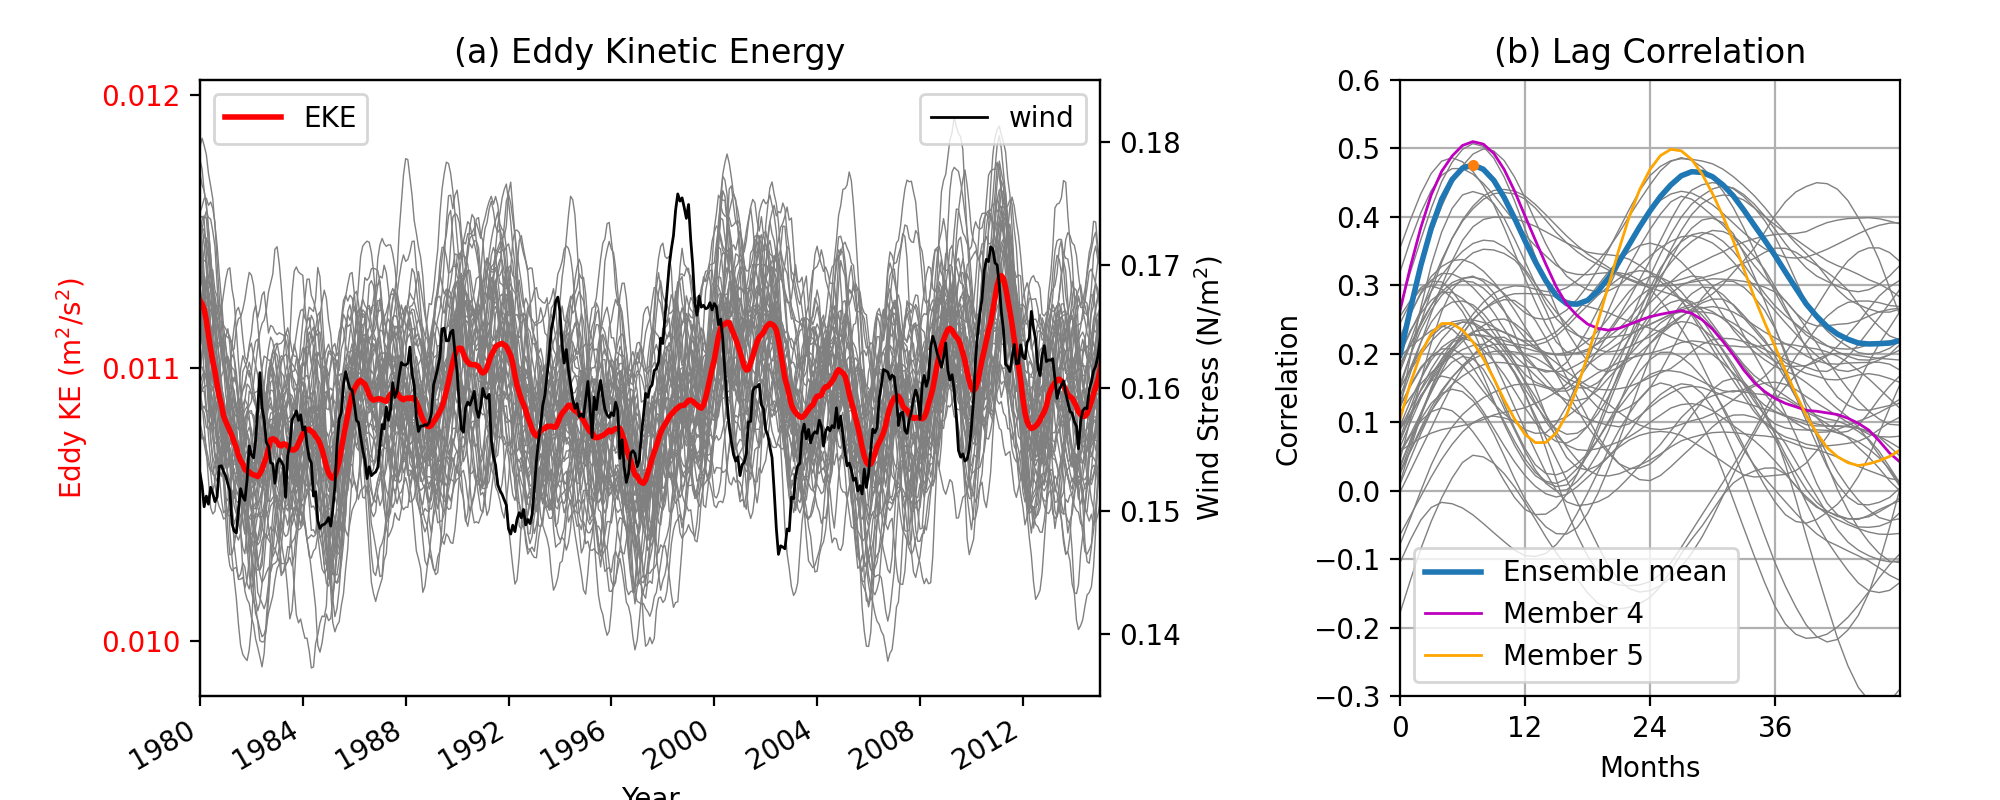
\includegraphics[width=\hsize]{Figure2}
\caption{Eddy kinetic energy statistics over the Southern Ocean (40$^\circ$S--60$^\circ$S). (a) Spatially averaged deseasonalised EKE anomaly (relative to climatology) for individual ensemble members (grey) and the ensemble mean (red) along with wind stress (black); and (b) Time-lagged correlation between wind stress and EKE for the ensemble mean (red) and individual ensemble  members (grey) -- with two individual ensemble members highlighted in magenta and orange.}
\label{Fig:2}
\end{center}
\end{figure}

Although Southern Ocean EKE variability is strongly intrinsic, there remains a component of forced variability (red line in Fig.~\ref{Fig:2}a).
Previous studies have suggested that there is a strong contribution of wind stress forcing upon EKE, and we therefore compare the forced variability with the variations in wind stress averaged over the same circumpolar belt (black line in Fig.~\ref{Fig:2}a).
This comparison suggests a relationship in which wind stress leads variations in EKE, consistent with previously published results.
However, the time-lagged correlations between wind stress and EKE suggests that this relationship is complex. 
The intrinsically variable nature of Southern Ocean eddies means that for some ensemble members, there is no meaningful correlation between wind stress and eddies (grey lines in Fig~\ref{Fig:2}b).
On the other hand, ensemble member 5 (magenta line) has a clear (and significant; $T = 5.5$) correlation with a 4-month lag, while member 25 (orange line) is weakly correlated at 6 months, and significantly correlated ($T = 4.2$) at a 24-month lag.
These isolated examples highlight the differing behaviour of each ensemble member. 
The ensemble mean (red line in Fig~\ref{Fig:2}b) includes a significant correlation at $\sim$4 months and a second significant peak at $\sim$30 months.
Thus, two distinct timescales of response of the Southern Ocean eddy field to wind stress are present in this model. 

\begin{figure}[t]
\begin{center}
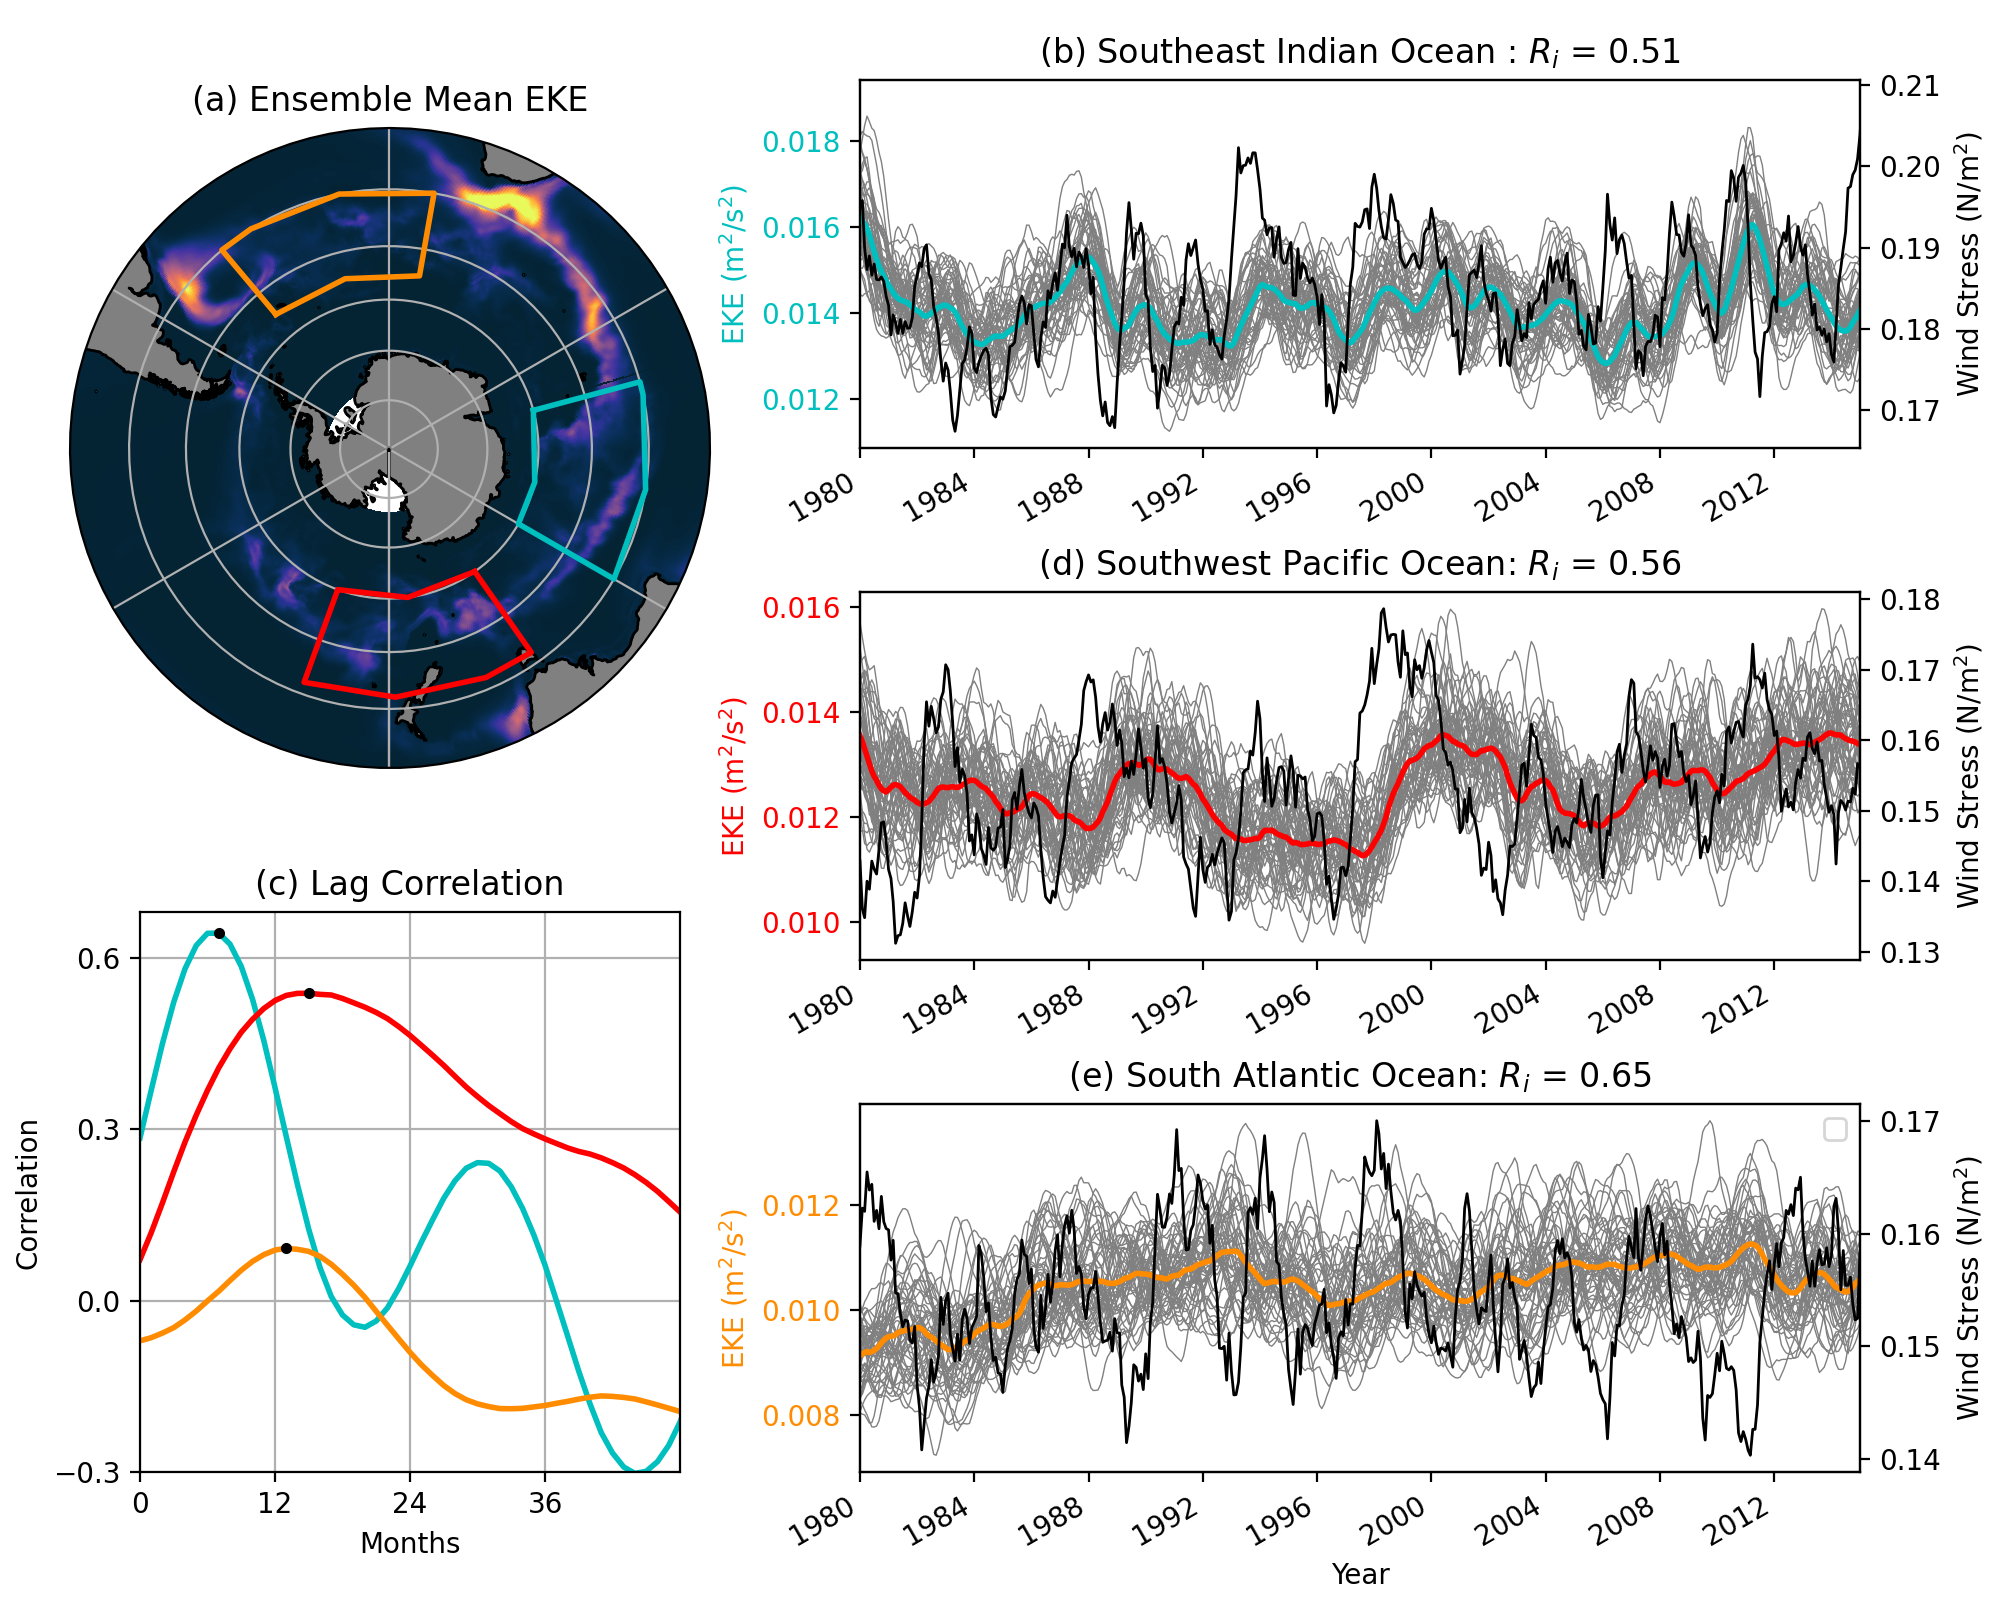
\includegraphics[width=\hsize]{Figure3}
\caption{Eddy kinetic energy statistics within sub-regions of the Southern Ocean. (a) Map showing Ensemble Mean EKE, along with 3 boxes over which a regional EKE analysis is applied; (b) Regional analysis of the Southeast Indian Ocean showing ensemble mean EKE in cyan, individual ensemble members EKE in grey and local wind stress averaged over the region in black; (c) Lagged correlation of ensemble mean EKE in each of the three regions; (d) Regional analysis of the Southwest Pacific Ocean showing ensemble mean EKE in red, individual ensemble members EKE in grey and local wind stress averaged over the region in black; and (c) Regional analysis of the South Atlantic Ocean showing ensemble mean EKE in orange, individual ensemble members EKE in grey and local wind stress averaged over the region in black. The fraction of intrinsic variance in each region is shown in the caption of panels (b), (d) and (e).}
\label{Fig:3}
\end{center}
\end{figure}

The ensemble of simulations shown here allow us to look in more detail at smaller regions of the Southern Ocean.
Calculating the variability of EKE in a smaller region has the advantage of isolating the individual processes which may occur in differing regions (for example, stronger topographic steering in places with steep bathymetry).
However, this advantage is partly offset by higher intrinsic variability;  if the region of interest is sufficiently small, then an individual eddy or event can have a large influence over the EKE timeseries.
In balancing these competing issues, we examine the variability within regions that span 15-20$^\circ$ in latitude and 30-40$^\circ$ in longitude, as shown in Figure \ref{Fig:3}(a).
We analyse the EKE timeseries averaged over these boxes -- including individual member EKE, ensemble mean EKE and lagged correlations between local wind stress forcing and the ensemble mean EKE in Fig. \ref{Fig:3}(b-e).

We first examine a region in the lee of Kerguelen Plateau in the Southeast Indian Ocean (cyan box in Fig.~\ref{Fig:3}a).
This region is characterised by high-frequency ($\sim$1 year) variations in EKE, with a relatively large forced component (the intrinsic variance fraction, $R_i = 0.63$, is smaller than the Southern Ocean average; Fig.~\ref{Fig:3}b).
The forced variation is clearly evident in the timeseries of  individual ensemble members; and this forced component is related to wind stress.
The lag between wind stress variations and ensemble mean EKE is short ($\sim$ 5 months; cyan line in Fig.~\ref{Fig:3}c) with a single clear  and significant peak in the lagged correlation.
There is a second, weaker but significant, correlation at 30 months lag.
This region highlights a regime in which the eddy field primarily responds rapidly to variations in the local wind stress.

In the Southeast Pacific Ocean (red box in Fig.~\ref{Fig:3}a) the situation is clearly different.
Here, the intrinsic variance fraction is larger than in the Southeast Indian Ocean ($R_i=0.78$) and the timescale of the variability is much longer; there is no significant response to wind stress variations which occur at sub-annual scales (Fig.~\ref{Fig:3}d).
The maximum values in the lag correlation occur over a broad band from 9-24 months in this region, without a single clear peak.
Thus, this region varies slowly and consistently to interannual variations in wind stress.

In the South Atlantic Ocean (orange box in Fig.~\ref{Fig:3}a) the system is again dominated by intrinsic variance ($R_i=0.74$) and is poorly correlated with wind stress forcing (Fig.~\ref{Fig:3}c,e), reinforcing the circumpolar variability of the EKE response to wind.
Other regions (see Fig. \ref{Fig:4}) highlight different aspects of the local eddy response;  with almost no correlation with wind forcing over the Central South Pacific ( Fig. \ref{Fig:4}b) or the Southwest Indian Ocean  (the Agulhas meander region; Fig. \ref{Fig:4}e).
In both of these regions, intrinsic variability dominates the signal and correlations are weak and insignificant. 
On the other hand, the Southeast Pacific (north of the main pathway of the ACC) shows a strong and coherent multi-year response to wind stress, with smaller intrinsic variance fraction and a peak lag at 30 months.
It is notable that this region, which is north of the mean ACC pathway, has a weak EKE signal (one tenth the magnitude of the core of the ACC).
The circumpolar variation in both EKE response times and intrinsic variability suggests that the two-timescale response seen in Fig. \ref{Fig:2} may be created by different processes, which each dominate in different regions of the Southern Ocean.


\begin{figure}[t]
\begin{center}
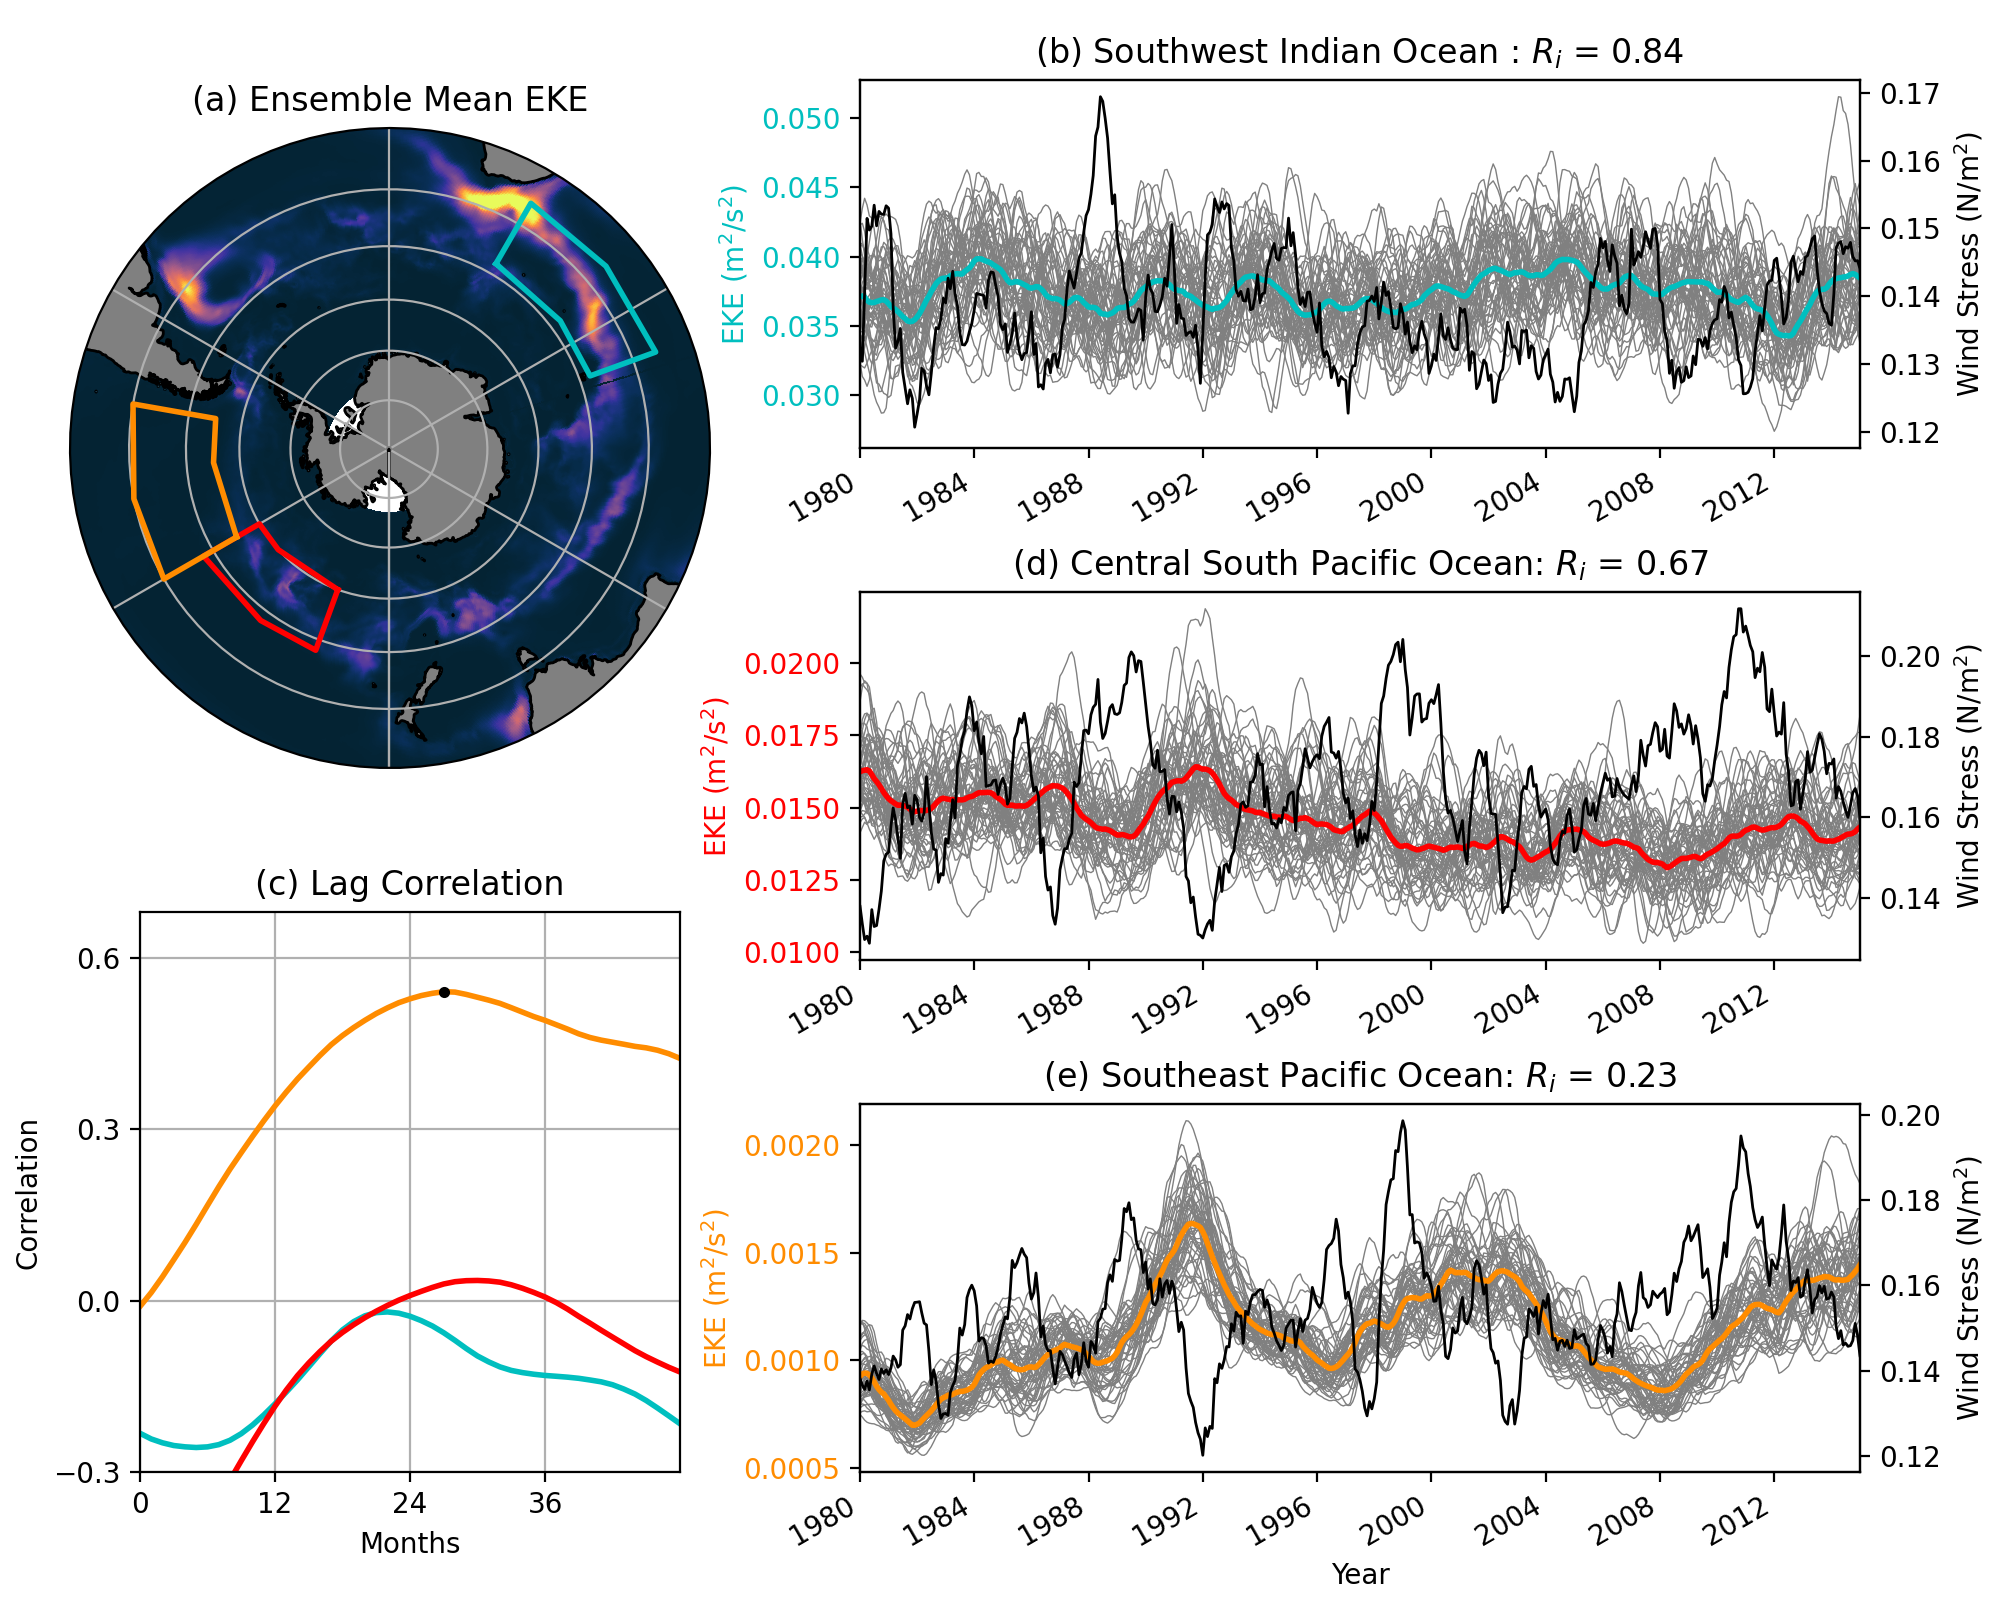
\includegraphics[width=\hsize]{Figure4}
\caption{Eddy kinetic energy statistics within sub-regions of the Southern Ocean. (a) Map showing Ensemble Mean EKE, along with 3 boxes over which a regional EKE analysis is applied; (b) Regional analysis of the Central South Pacific Ocean showing ensemble mean EKE in cyan, individual ensemble members EKE in grey and local wind stress averaged over the region in black; (c) Lagged correlation of ensemble mean EKE in each of the three regions; (d) Regional analysis of the Southeast Pacific Ocean showing ensemble mean EKE in red, individual ensemble members EKE in grey and local wind stress averaged over the region in black; and (e) Regional analysis of the Southwest Indian  Ocean showing ensemble mean EKE in orange, individual ensemble members EKE in grey and local wind stress averaged over the region in black. The fraction of intrinsic variance in each region is shown in the caption of panels (b), (d) and (e).}
\label{Fig:4}
\end{center}
\end{figure}



\begin{figure}[t]
\begin{center}
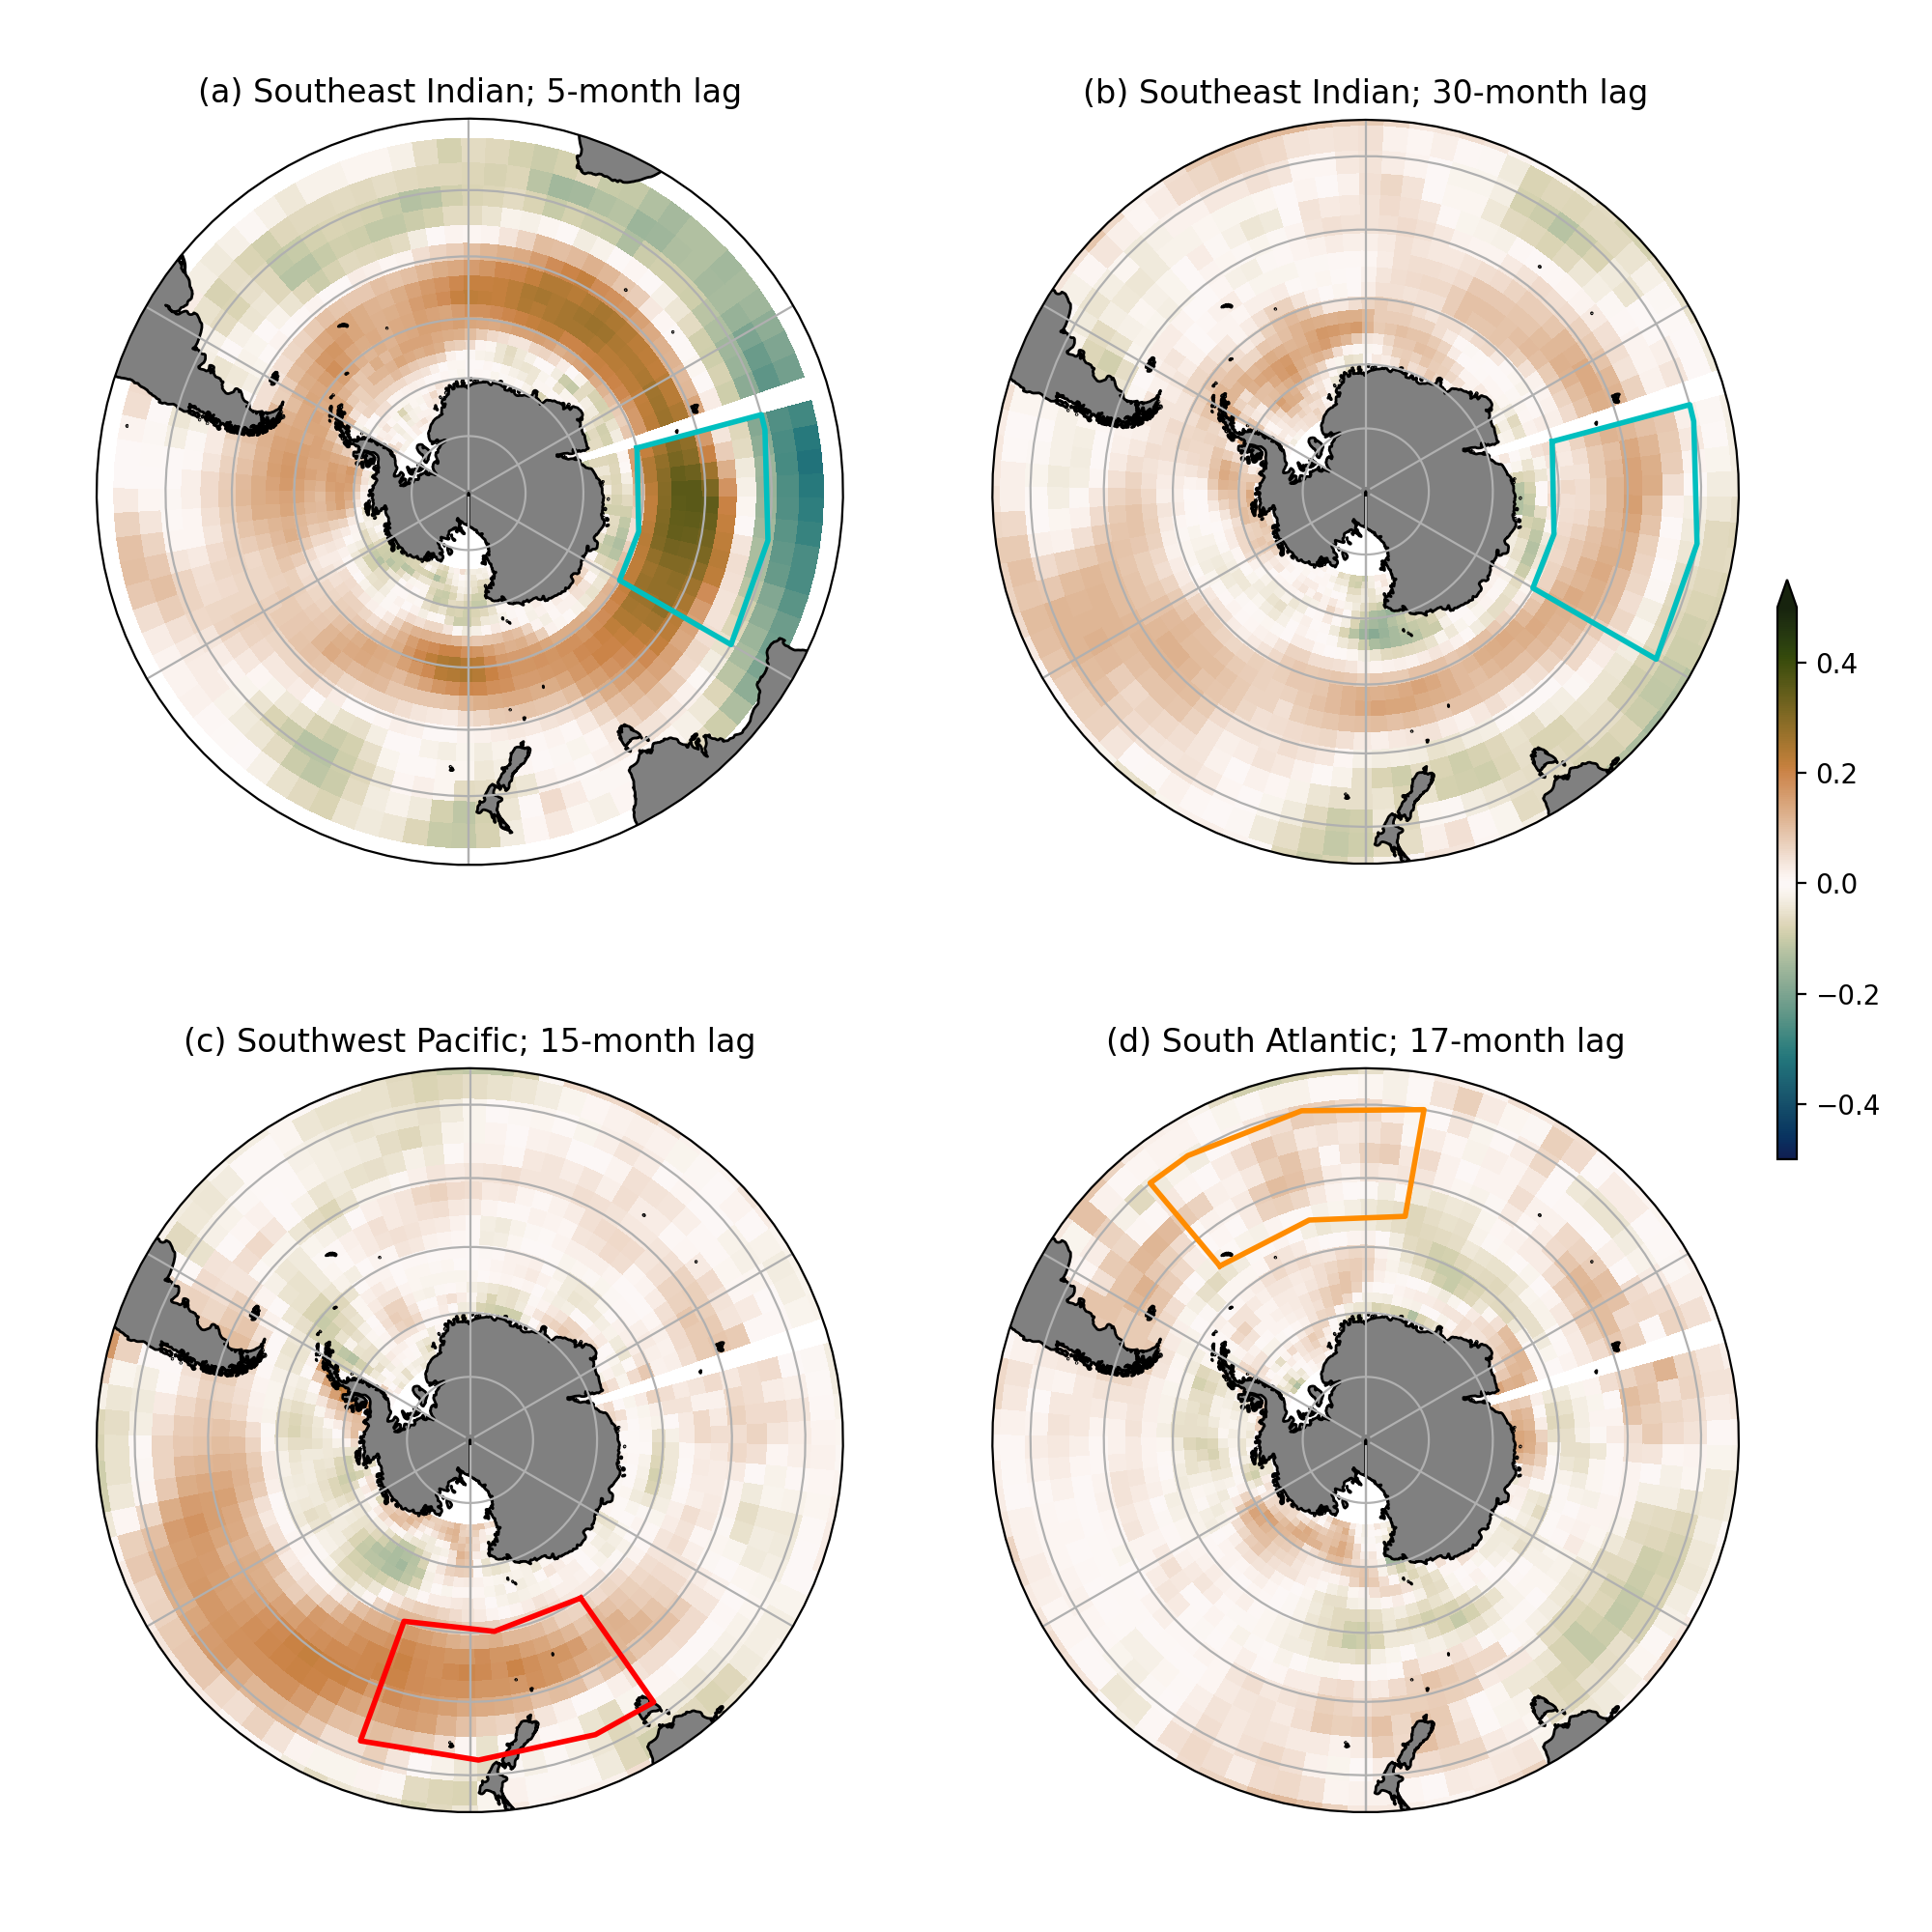
\includegraphics[width=\hsize]{Figure5}
\caption{The spatial correlation of wind stress with $\langle\textrm{EKE}\rangle$ in (a) the Southeast Indian Ocean at 5-month lag; (b) the Southeast Indian Ocean at 30-month lag; (c) the Southwest Pacific ocean at 15-month lag and (d) the South Atlantic Ocean at 17-month lag.}
\label{Fig:5}
\end{center}
\end{figure}

The heterogeneity in correlations between local wind and the ensemble-mean EKE ($\langle\textrm{EKE}\rangle$) shows that, where forced variability in Southern Ocean EKE occurs, it can be partly explained by variations in wind stress.
However, these correlations are based purely on local wind stress -- averaged over the same area as the EKE statistics.
The existence of multi-year lags between the wind and the EKE suggests that local winds may not be the only source of energy for eddy generation; in particular, it is possible that energy could be advected a considerable distance downstream during this lag period.
To investigate this question we now take each of the regions outlined in Fig. \ref{Fig:3} and look at the spatial correlation between wind stress and the local ensemble mean EKE (Fig. \ref{Fig:5}).
To make this calculation, wind stress is first coarsened to a 4$^\circ \times $4$^\circ$ grid, and wind stress in each of those coarsened grid cells correlated with ensemble-mean EKE at different lags.
In the Southeast Indian Ocean, Fig.~\ref{Fig:3}(c) shows correlation maxima at 5 months and 30 months; the spatial variation of this correlation is shown in Fig. \ref{Fig:5}(a,b) respectively.
These figures highlight a key feature of Southern Ocean wind stress, which is that there are strong autocorrelations between wind stress along a line of latitude; nonetheless, the maximum correlation between wind stress and $\langle\textrm{EKE}\rangle$ occurs within the $\langle\textrm{EKE}\rangle$-averaging region.
This correlation is lower in magnitude at 30 months (consistent with Fig.~\ref{Fig:3}c), but at both 5 and 30 month lags the correlation with wind upstream of the $\langle\textrm{EKE}\rangle$-averaging region is not stronger than within the $\langle\textrm{EKE}\rangle$-averaging region.
A similar result is found in the Southwest Pacific Ocean (Fig.~\ref{Fig:5}c); wind stress correlations are relatively uniform across the Pacific Ocean owing to the autocorrelation of winds, but the correlations are less circumpolar than the Southeast Indian Ocean.
Importantly, there is no suggestion of a strong correlation with wind stress upstream of the $\langle\textrm{EKE}\rangle$-averaging region.
In the South Atlantic, the $\langle\textrm{EKE}\rangle$ is not strongly correlated with wind stress, either in the local region or elsewhere in the Southern Ocean (Fig.~\ref{Fig:5}d).
Thus, these spatial maps demonstrate that, where strong forced variability in the $\langle\textrm{EKE}\rangle$ exists, it is most strongly linked to local wind stress, with no suggestion of upstream or remote wind input playing a strong role. 

\section{Discussion and Conclusions}
The simulations shown here advocate for a probabilistic approach to understanding the Southern Ocean eddy field.
The 50-member ensemble of eddy-permitting ocean-sea ice model simulations investigated here demonstrate that inference about the EKE response of a single ensemble member to variable forcing in a localised region is not robust, consistent with the inference of \citet{Zhang2021}.
This point is clarified in Fig.~\ref{Fig:6} which shows a map of the intrinsic fraction of variance, $R_i$, from eddy statistics interpolated onto a coarse 5$^\circ \times$5$^\circ$ grid.
Here, the chaotic variance dominates over most of the band of elevated EKE in the Southern Ocean. 
Subpanels (b) and (c) confirm the predominance of intrinsic eddy variability at this scale, highlighting that at small scales we can place little reliability on the results from an individual ensemble member, or a single observation.

\begin{figure}[t]
\begin{center}
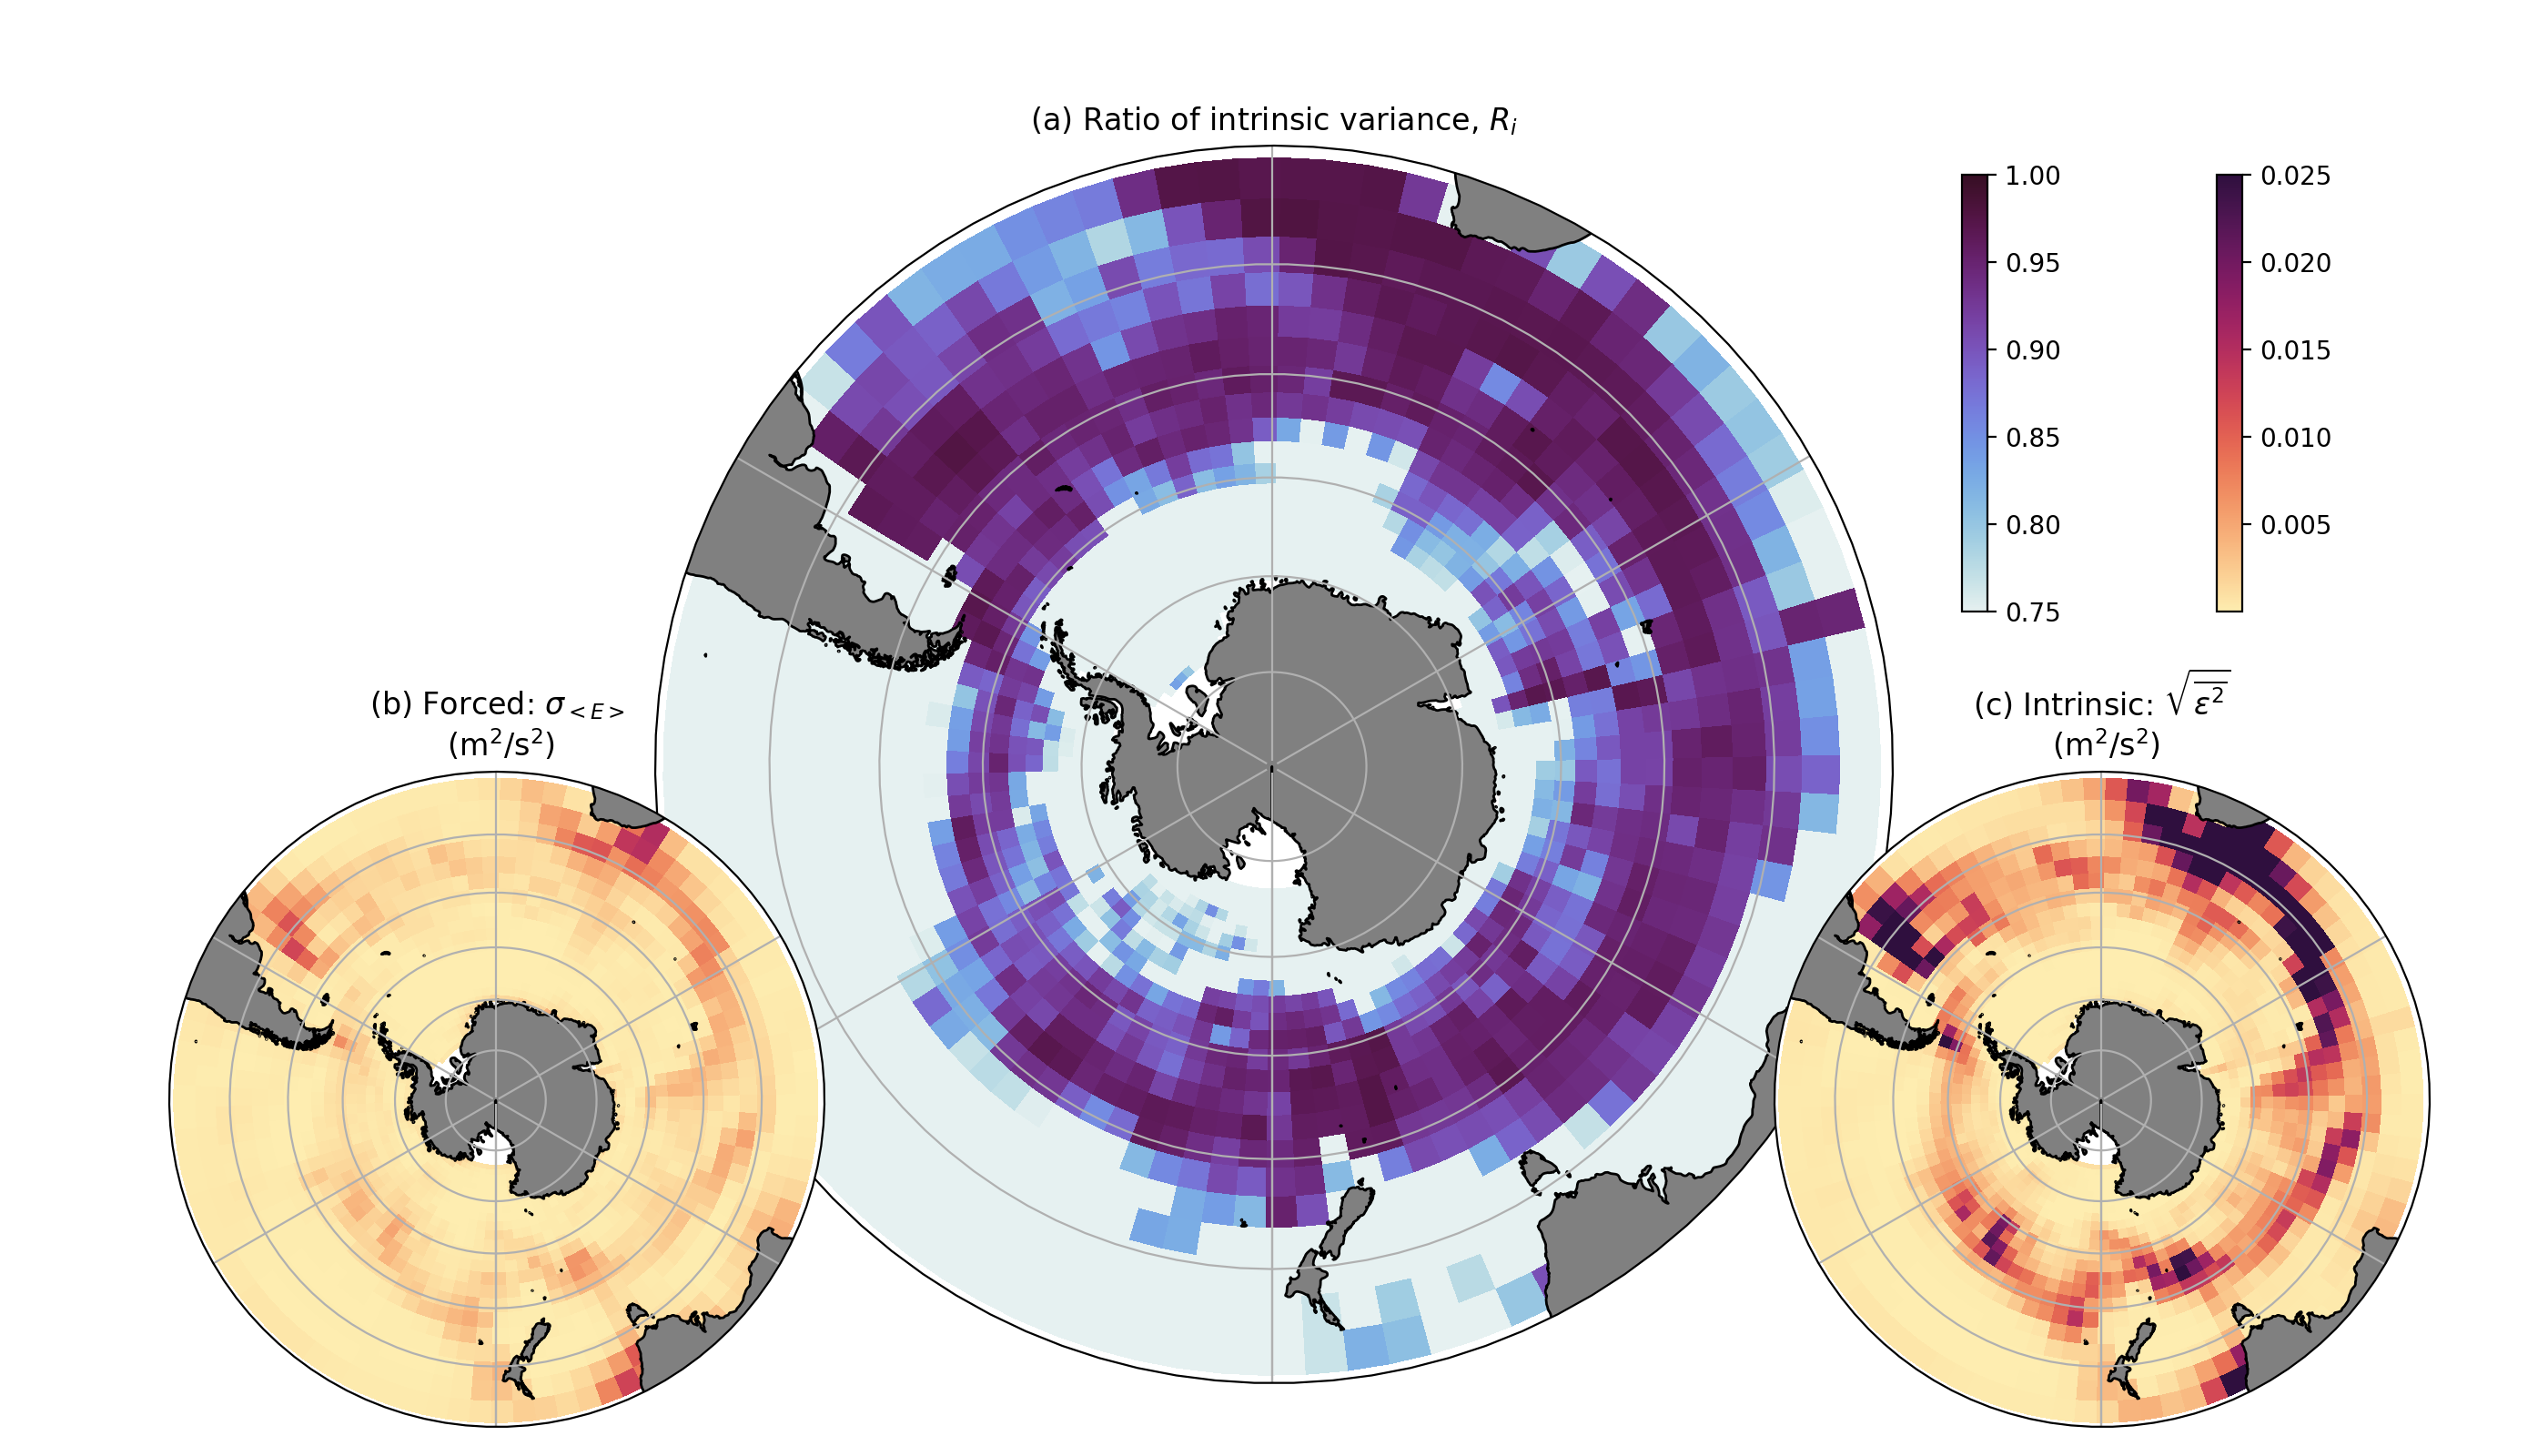
\includegraphics[width=\hsize]{Figure6}
\caption{(a) The intrinsic variance fraction, $R_i$, averaged onto a  5$^\circ \times$5$^\circ$ grid; (b) amplitude of variability due to forced processes and (c) amplitude of variability due to intrinsic processes. {\color{red}(Thierry: How about adding to this figure the same 3 maps for the interannual EKE variability alone? This would explicitly show that intrinsic signals remain strong even at low-frequencies: this can be explicitly stated in the text.)}}
\label{Fig:6}
\end{center}
\end{figure}

When averaged over larger regions, the fraction of intrinsic variance can be smaller than shown in Fig.~\ref{Fig:6}.
For example, in the Southeast Indian Ocean, in the lee of the Kerguelen Plateau, a strong and rapid response of EKE to the local wind stress can be observed.
On the other hand, slower but significant responses in EKE are found in the Southwest Pacific Ocean, near Campbell Plateau (Fig.~\ref{Fig:3}).
Both of these regions are locations where topography acts to sharpen and energise fronts.
However, in many other regions, EKE variability appears to be almost entirely chaotic.
This heterogeneity, consistent with the findings of \citet{Patara2016}, acts to emphasise the differing flow regimes which are found in different parts of the Southern Ocean.

Averaged over the entire Southern Ocean two significant timescales of correlation are found between wind stress and $\langle\textrm{EKE}\rangle$: one at 4 months, and the other at $\sim$30 months.
The rapid timescale is the expected Ekman response, in which wind stress tilts isopycnals to store available potential energy, which is then released to EKE through baroclinic instability \citep[e.g.][]{Sinha2016}.
The slower timescale is similar to that proposed by \citet{Meredith-Hogg-2006}, based on the single large Southern Ocean wind event in 1999.
This timescale is consistent with the  topographic feedback mechanism of \citet{Hogg-Blundell-2006}, in which a delayed amplification of the EKE response can occur through the topographic steering of currents away from the zonal direction, which decreases the stability of the current.
 
The ensemble approach thus leads to the conclusion that eddy processes in the Southern Ocean include a large component of chaotic variability, even when averaged over a large spatial area and up to interannual time scales.
This result argues for caution in interpreting observations of Southern Ocean eddies, which are necessarily based on a single, short realisation of the natural world.
Given that eddies are critical for the Southern Ocean circulation, this result implies that predictability of the future Southern Ocean may be weaker than previously thought.
It also highlights the difficulty faced in distinguishing the processes that govern eddy dynamics in this system, and point to more systematic eddy identification and modelling studies to better isolate these processes.
 


\acknowledgments
This research was undertaken with the assistance of resources and services from the National Computational Infrastructure (NCI), which is supported by the Australian Government.
AMH is gratefully to the MEOM team at ICE, Universit{\'e} Grenoble Alpes, who supported his sabbatical and which led to this work. 
The results of this research have been achieved using the PRACE Research Infrastructure resource CURIE based in France at TGCC. 
This work is a contribution to the OCCIPUT and PIRATE projects. 
OCCIPUT has been funded by ANR through contract ANR-13-BS06-0007-01. 
PIRATE has been funded by CNES through the Ocean Surface Topography Science Team (OST-ST). 
{\color{red}The model output used in this study can be downloaded from the Zenodo repository at doi:XXX.XXX.XXX.}
The full OCCIPUT model dataset is available on request (\href{mailto:Thierry.Penduff@cnrs.fr}{Thierry.Penduff@cnrs.fr}).

\bibliography{references}

\end{document}
